\documentclass[12]{article}
 \usepackage{german}
 \usepackage{epsfig}
 \usepackage{graphics}
 \usepackage{color}
  \newcommand{\cor}[1]{{\color{red}#1}}
\begin{document}

\textbf{Redefinition of distances and angles for  AMOR}

J. Stahn, \today
\vfill

This is a description how to calculate the instrument geometry for
differing inputs of mom (monochormator omega), som (sample omega) and
s2t (sample two theta). 

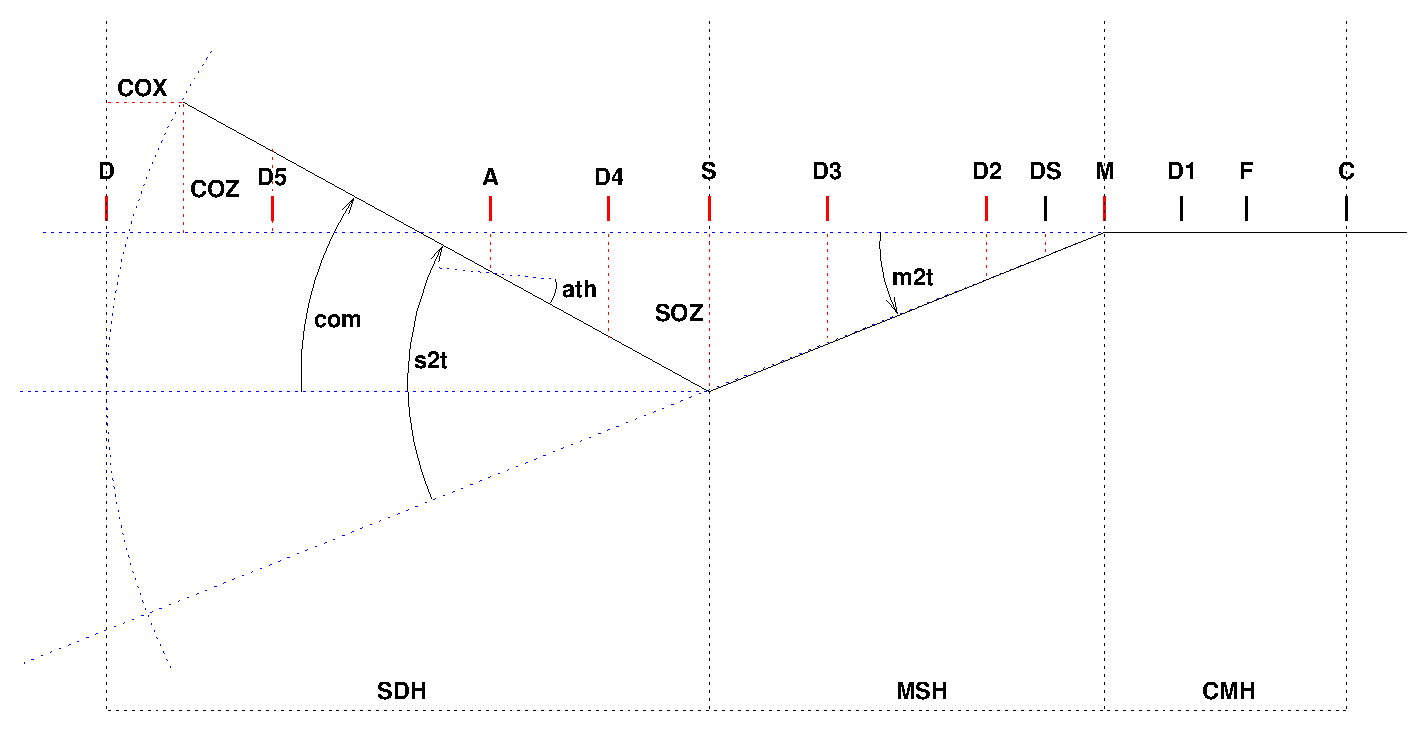
\includegraphics[width=\textwidth]{distances.eps}
\vfill

\begin{tabular}{ll}
 $\sf C   $ & chopper \\
 $\sf F   $ & Filter \\
 $\sf M   $ & Monochromator / Polarisator \\
 $\sf S   $ & sample \\
 $\sf A   $ & Analysator  \\
 $\sf D   $ & Detektor \\
 $\sf D_x $ & Blende $x$ \\
\end{tabular} \\

The zeropoint is  $\sf C$ at beam height \\

Every horizontal position will be read from a scale on the granite
base of the instrument.  \\
Example: $\sf S$: At the foot of the sample table there is a mark for
reading. You read the value $\sf S'$. 
This value has the known distance  to true $\sf S$.
I addition the scale is running in the wrong direction with a
zeropoint at  $d = ???? \,\mathrm{mm}$. Thus: \\
${\sf S} = d - {\sf S'} - l_{\sf S}$ \\

Thus we need a static table which contains all $d$ 
and all $l_{\sf I}$. In addition we need a  dynamic table holding the
values$\sf I'$. In future we will read thos values through an
encoder. Actually (2016) this is a laser distance measuring system.





\cor{red}: Values to be choosen by the user, inputs \hfill
\textsf{small}: Angles \hfill
\textsf{CAPITALS}: distances
\begin{eqnarray}
 \sf \cor{mom} & & \\[2ex]
 \sf \cor{som} & & \\[1ex]
 \sf \cor{STZ} & & \\[1ex]
 \sf SOZ  &=&\sf  MSH \tan[ \cor{-m2t} ] \\[2ex]
 \sf com  &=&\sf  \cor{s2t} - \cor{m2t} \\[1ex]
 \sf COX  &=&\sf  - SDH \, \left( \cos[ com ] - 1 \right) \\[1ex]
 \sf COZ  &=&\sf  SOZ + SDH \, \sin[ com ] \\[1ex]
 \sf \cor{C3Z} & & \\[3ex]
 \sf D_SB &=&\sf  MB_S \, \tan[ \cor{-m2t} ] - 10 \\[1ex]
 \sf D_2B &=&\sf  MD_2 \, \tan[ \cor{-m2t} ] - 0.5 \, \cor{D_2T} \\[1ex]
 \sf D_3B &=&\sf  MD_3 \, \tan[ \cor{-m2t} ] - 0.5 \, \cor{D_3T} \\[1ex]
 \sf D_4B &=&\sf  SOZ + SD_4 \, \tan[ com ] - 0.5 \, \cor{D_4T} \\[2ex]
 \sf D_5B &=&\sf  SOZ + SD_5 \, \tan[ com ] - 0.5 \, \cor{D_5T} \\[2ex]
 \sf AOZ  &=&\sf  SOZ + SA \, \tan[ com ] \\[1ex]
 \sf aom  &=&\sf  com + \cor{ath} \\[2ex]
 \sf CD   &=&\sf  CMH + \sqrt{SMH^2 + SOZ^2} + SDH    
\end{eqnarray}


\end{document}
